\subsubsection{Dubey's patterns}\label{sec:dubey}
%see https://www.researchgate.net/profile/Anshu_Dubey3
%ref~\cite{Du16Idea, Du19divi}

There are many well-documented software development processes, such as waterfall, spiral,
rapid application development (RAD) and agile.
The purpose of these processes is to decompose software development into its
constituent components, so that developers can focus on the
quality of each component separately, raising the quality of the software
overall.
Dubey and McInnes \cite{Du16Idea} discuss software lifecycle processes in the
context of scientific software development.
They note that, in contrast to most non-scientific software development where
the goal is software creation, in scientific software development, software is
the \emph{means} of conducting research, not the \emph{product} of it.
Therefore they argue that conventional processes of software development are not
well-suited to scientific software development.

In \cite{Du16Idea}, Dubey and McInnes describe a scientific software lifecycle,
formalizing the approaches already used in various projects, such as
SAMRAI \cite{SAMRAI}, FLASH \cite{Du09Exte}, Enzo \cite{Br14ENZO} and Amanzi
\cite{Mo14Aman}.
The key point is that scientific software can be thought of as consisting of
two components:
the \emph{infrastructure} code 
and the \emph{scientific capability} code.
The infrastructure code handles tasks like discretizations and I/O.
It is relatively stable, and it may be developed using any standard software
lifecycle pattern.
The scientific capability code describes the scientific model itself.
Its requirements are research-driven, and the code itself is constantly
evolving.
Dubey and McInnes introduce a software development lifecycle for the scientific
capability code, and describe how this should interface with the
development process of the infrastructure code.
Isolating the scientific code from the infrastructure code and limiting the
points of contact between them allows rapid prototyping and development of
scientific code, without undermining the stability or functionality of
infrastructure code.

\paragraph{Scientific capability development process}

The development lifecycle proposed by Dubey and McInnes is shown schematically in
Figure \ref{fig:DubeyFigs}(a).
The essential components are connected by solid lines.
The process is this:
first, requirements for the software are gathered, and the target phenomena are
described using a mathematical model.
Next, approximations are introduced as necessary to simplify the model or make
it tractable.
Then the equations are discretized, and appropriate numerical algorithms
implemented to solve the model.
The resulting software is then tested for correctness -- \emph{i.e.}\ that is
solves the correct equations -- and its stability and convergence properties
are studied.
This produces software of the required standard, but it does not ensure that
the underlying mathematical model adequately describes the target phenomena.
The code is therefore then validated against calibrated observations, with the
mathematical model feeding into the calibration by defining regimes in which
the model is valid.
The validation phase then feeds back into the approximation, algorithm and
(occasionally) the discretization phases, if it is necessary to make changes
to ensure that the model describes the target phenomena.
This feedback from simulations into planning is an integral part of the
evolution of scientific code requirements capture.

\begin{figure}[thp]
(a)\centerline{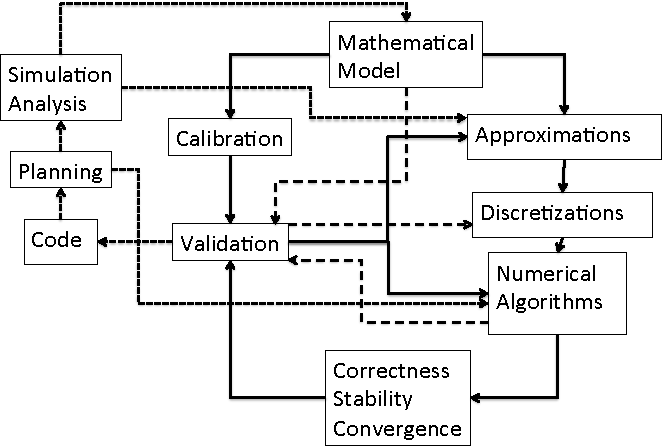
\includegraphics[width=0.8\textwidth]{../png/DubeyFig3.png}}
\\(b)\centerline{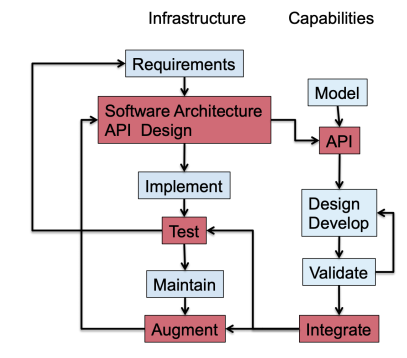
\includegraphics[width=0.8\textwidth]{../png/wkflow.png}}
	\caption{Lifecycle patterns proposed by Dubey and McInnes \cite{Du16Idea}: 
	(a) the scientific software lifecycle pattern; and
	(b) the interaction of the infrastructure and scientific capability patterns.
	These graphics are respectively Figures 3~and~4 of ref~\protect{\cite{Du16Idea}},
        the latter also corresponds to Figure~1 of ref~\protect{\cite{y1re311}}. \label{fig:DubeyFigs}}
\end{figure}

The wide-dashed arrows from mathematical models and numerical algorithms
indicate phases that may be skipped in certain cases.
For example, calibration may not be needed in simple cases where a
mathematical model is universally applicable.
Similarly, some correctness, stability and convergence checks may not be
required if the software uses third-party libraries or externally-verified
software suites.

Finally, the narrow-dashed lines indicate how the software development cycle interfaces
with other concerns like simulation planning and scientific developments in the
field.
Planning, such as determining available compute resources can necessitate
changes to the numerical implementation to make a set of simulations feasible.
Analysis of simulation results can lead to an improved understanding of the
target phenomena, which can result in modifications to the mathematical model
and approximations used.

The above description treats a single mathematical model.
In more complex multiscale or multiphysics systems, there will be multiple
mathematical models, but the same software lifecycle may be used for each model
independently.

\paragraph{Interfacing development processes}
Now we must consider how to connect the development process for scientific capability code
described above with a standard development process used for infrastructure code.
Ideally, there will be few points of contact between the two processes, as this
will allow separation of concerns, and for the two software lifecycles to
proceed at their differing rates largely independent of one another.
Dubey and McInnes \cite{Du16Idea} propose the approach shown in Figure\
\ref{fig:DubeyFigs}(b), where high-level descriptions of the infrastructure and
scientific capability codes are given in the left- and right-hand columns
respectively.
There are only three coupling points between the two lifecycles.
The primary coupling point is through the design of the API.
A well-designed module structure will ensure that discrete modules
communicate their data through a fairly stable API.
However, improvements in scientific understanding might reveal necessary
changes in the data dependencies between modules, that would be reflected in
changes to the API.
The other coupling points are where the scientific capability code interfaces
with the infrastructure's testing framework,
and where improving the scientific capability of the code (by perhaps adding
a feature) means that the functionality of infrastructure code must also be
extended.
These coupling points are however very limited, and therefore the
infrastructure and scientific capability code can be developed with largely
independent lifecycles.
